% move all configuration stuff into includes file so we can focus on the content
\documentclass[aspectratio=169,hyperref={pdfpagelabels=false,colorlinks=true,linkcolor=white,urlcolor=blue},t]{beamer}

%%%%%%%%%%%%%%%%%%%%%%%%%%%%%%%%%%%%%%%%%%%%%%%%%%%%%%%%%%%%%%%%%%%%%%%%%%%%%%%%%%
%%%%%%%%%%%%%%%%%%%%%%%%%%%%%%%%%%%%%%%%%%%%%%%%%%%%%%%%%%%%%%%%%%%%%%%%%%%%%%%%%%
% packages
\usepackage{pict2e}
\usepackage{epic}
\usepackage{amsmath,amsfonts,amssymb}
\usepackage{units}
\usepackage{fancybox}
\usepackage[absolute,overlay]{textpos} 
\usepackage{media9} % avi2flv: "C:\Program Files\ffmpeg\bin\ffmpeg.exe" -i TuneFreqFilterbank.avi -b 600k -s 441x324 -r 15 -acodec copy TuneFreqFilterbank.flv
\usepackage{animate}
\usepackage{gensymb}
\usepackage{multirow}
\usepackage{silence}
\usepackage[backend=bibtex,style=ieee]{biblatex}
\AtEveryCitekey{\iffootnote{\tiny}{}}
\addbibresource{references}

%%%%%%%%%%%%%%%%%%%%%%%%%%%%%%%%%%%%%%%%%%%%%%%%%%%%%%%%%%%%%%%%%%%%%%%%%%%%%%%%%%
%%%%%%%%%%%%%%%%%%%%%%%%%%%%%%%%%%%%%%%%%%%%%%%%%%%%%%%%%%%%%%%%%%%%%%%%%%%%%%%%%%
% relative paths
\graphicspath{{graph/}}


%%%%%%%%%%%%%%%%%%%%%%%%%%%%%%%%%%%%%%%%%%%%%%%%%%%%%%%%%%%%%%%%%%%%%%%%%%%%%%%%%%
%%%%%%%%%%%%%%%%%%%%%%%%%%%%%%%%%%%%%%%%%%%%%%%%%%%%%%%%%%%%%%%%%%%%%%%%%%%%%%%%%%
% units
\setlength{\unitlength}{1mm}

%%%%%%%%%%%%%%%%%%%%%%%%%%%%%%%%%%%%%%%%%%%%%%%%%%%%%%%%%%%%%%%%%%%%%%%%%%%%%%%%%%
%%%%%%%%%%%%%%%%%%%%%%%%%%%%%%%%%%%%%%%%%%%%%%%%%%%%%%%%%%%%%%%%%%%%%%%%%%%%%%%%%%
% theme & layout
\usetheme{Frankfurt}
\beamertemplatenavigationsymbolsempty
%\setbeamertemplate{frametitle}[smoothbars theme]
\setbeamertemplate{frametitle}
{
    \begin{beamercolorbox}[ht=1.8em,wd=\paperwidth]{frametitle}
        \vspace{-.1em}%
        \hspace{.2em}{\strut\insertframetitle\strut}
        
        \hspace{.2em}\small\strut\insertframesubtitle\strut
        %\hfill
        %
\includegraphics[height=.8cm,keepaspectratio]{CenterMusicTechnology-solid-2lines-white-CoAtag}
        
    \end{beamercolorbox}
    \begin{textblock*}{100mm}(11.6cm,.7cm)
        \includegraphics[height=.8cm,keepaspectratio]{logo_GTCMT_black}
    \end{textblock*}
}

% set this to ensure bulletpoints without subsections
\usepackage{remreset}
\makeatletter
\@removefromreset{subsection}{section}
\makeatother
\setcounter{subsection}{1}

%---------------------------------------------------------------------------------
% appearance
\setbeamercolor{structure}{fg=gtgold}
\setbeamercovered{transparent} %invisible
\setbeamercolor{bibliography entry author}{fg=black}
\setbeamercolor*{bibliography entry title}{fg=black}
\setbeamercolor*{bibliography entry note}{fg=black}

%\usepackage{pgfpages}
%\setbeameroption{show notes}
%\setbeameroption{show notes on second screen=right}
%---------------------------------------------------------------------------------
% fontsize
\let\Tiny=\tiny

%%%%%%%%%%%%%%%%%%%%%%%%%%%%%%%%%%%%%%%%%%%%%%%%%%%%%%%%%%%%%%%%%%%%%%%%%%%%%%%%%%
%%%%%%%%%%%%%%%%%%%%%%%%%%%%%%%%%%%%%%%%%%%%%%%%%%%%%%%%%%%%%%%%%%%%%%%%%%%%%%%%%%
% warnings
\pdfsuppresswarningpagegroup=1
\WarningFilter{biblatex}{Patching footnotes failed}
\WarningFilter{latexfont}{Font shape}
\WarningFilter{latexfont}{Some font shapes}
\WarningFilter{gensymb}{Not defining}


%%%%%%%%%%%%%%%%%%%%%%%%%%%%%%%%%%%%%%%%%%%%%%%%%%%%%%%%%%%%%%%%%%%%%%%%%%%%%%%%%%
%%%%%%%%%%%%%%%%%%%%%%%%%%%%%%%%%%%%%%%%%%%%%%%%%%%%%%%%%%%%%%%%%%%%%%%%%%%%%%%%%%
% title information
\title[]{Introduction to Audio Content Analysis}   
\author[alexander lerch]{alexander lerch} 
%\institute{~}
%\date[Alexander Lerch]{}
\titlegraphic{\vspace{-16mm}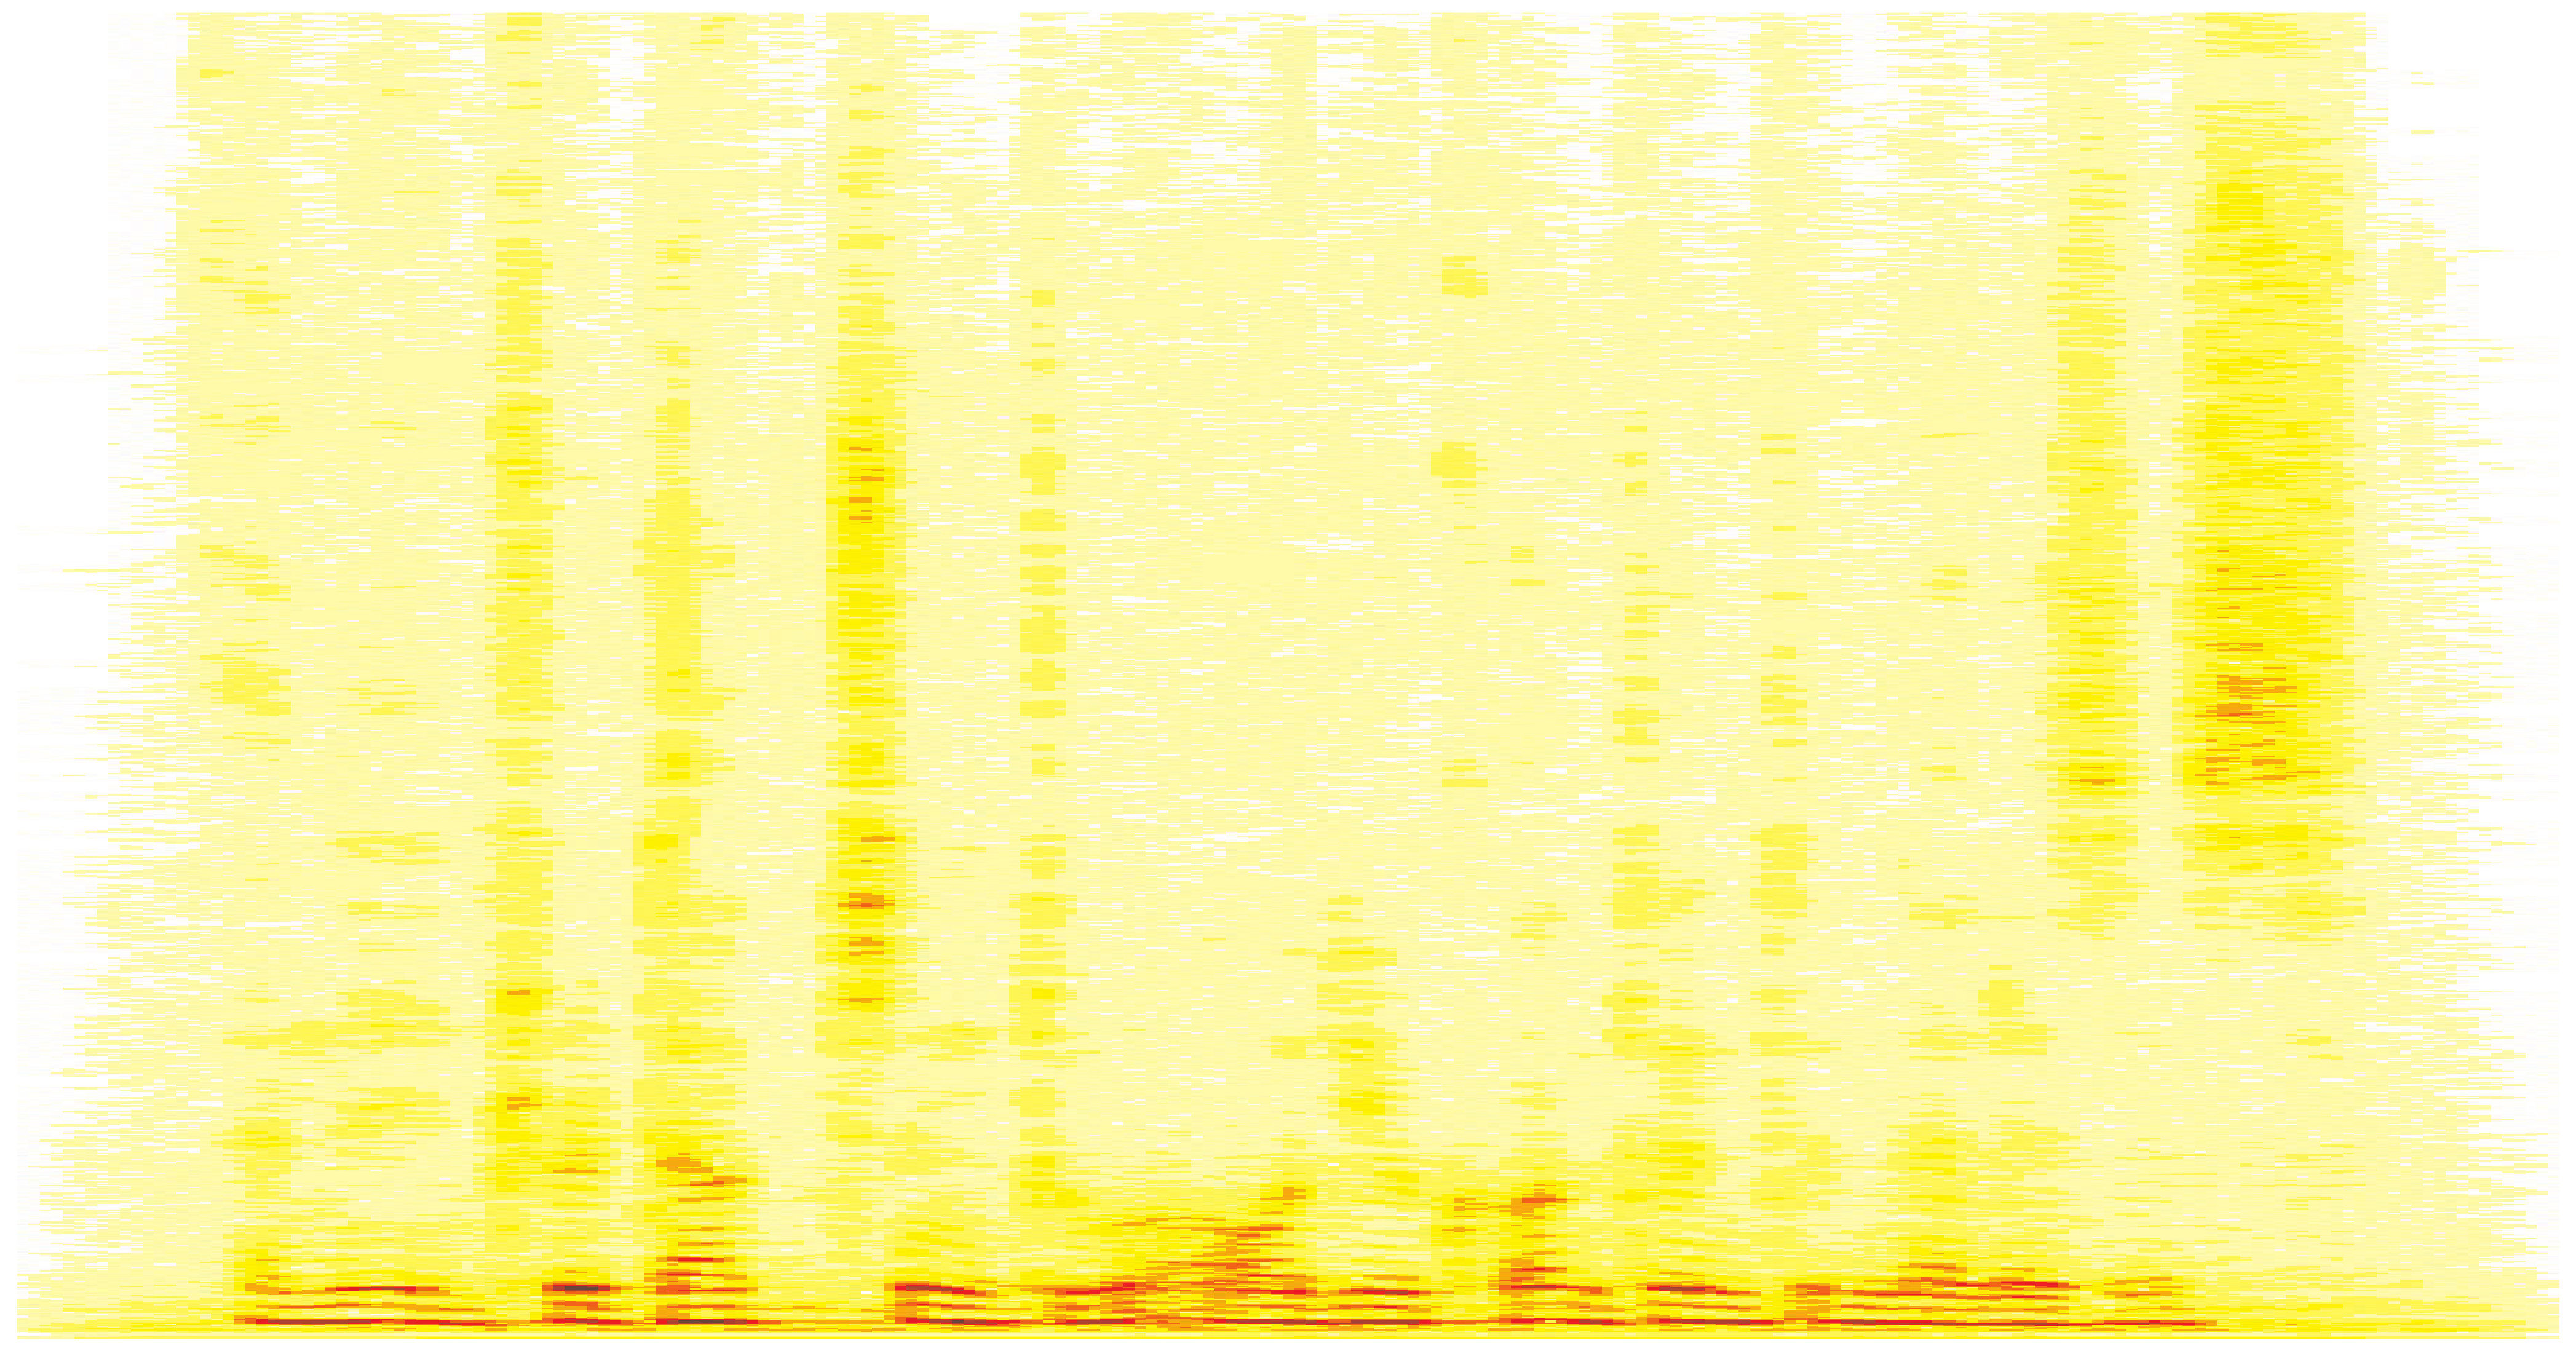
\includegraphics[width=\textwidth,height=3cm]{title}}

%%%%%%%%%%%%%%%%%%%%%%%%%%%%%%%%%%%%%%%%%%%%%%%%%%%%%%%%%%%%%%%%%%%%%%%%%%%%%%%%%%
%%%%%%%%%%%%%%%%%%%%%%%%%%%%%%%%%%%%%%%%%%%%%%%%%%%%%%%%%%%%%%%%%%%%%%%%%%%%%%%%%%
% colors
\definecolor{gtgold}{HTML}{E0AA0F} %{rgb}{0.88,0.66,1,0.06} [234, 170, 0]/256

%%%%%%%%%%%%%%%%%%%%%%%%%%%%%%%%%%%%%%%%%%%%%%%%%%%%%%%%%%%%%%%%%%%%%%%%%%%%%%%%%%
%%%%%%%%%%%%%%%%%%%%%%%%%%%%%%%%%%%%%%%%%%%%%%%%%%%%%%%%%%%%%%%%%%%%%%%%%%%%%%%%%%
% math
\DeclareMathOperator*{\argmax}{argmax}
\DeclareMathOperator*{\argmin}{argmin}
\DeclareMathOperator*{\atan}{atan}
\DeclareMathOperator*{\arcsinh}{arcsinh}
\DeclareMathOperator*{\sign}{sign}
\DeclareMathOperator*{\tcdf}{tcdf}
\DeclareMathOperator*{\si}{sinc}
\DeclareMathOperator*{\princarg}{princarg}
\DeclareMathOperator*{\arccosh}{arccosh}
\DeclareMathOperator*{\hwr}{HWR}
\DeclareMathOperator*{\flip}{flip}
\DeclareMathOperator*{\sinc}{sinc}
\DeclareMathOperator*{\floor}{floor}
\newcommand{\e}{{e}}
\newcommand{\jom}{\mathrm{j}\omega}
\newcommand{\jOm}{\mathrm{j}\Omega}
\newcommand   {\mat}[1]    		{\boldsymbol{\uppercase{#1}}}		%bold
\renewcommand {\vec}[1]    		{\boldsymbol{\lowercase{#1}}}		%bold

%%%%%%%%%%%%%%%%%%%%%%%%%%%%%%%%%%%%%%%%%%%%%%%%%%%%%%%%%%%%%%%%%%%%%%%%%%%%%%%%%%
%%%%%%%%%%%%%%%%%%%%%%%%%%%%%%%%%%%%%%%%%%%%%%%%%%%%%%%%%%%%%%%%%%%%%%%%%%%%%%%%%%
% media9
\newcommand{\includeaudio}[1]{{\includemedia[
                        addresource=audio/#1.mp3,
                        width=5mm,
                        height=5mm,
                        activate=onclick,
                        flashvars={
                            source=audio/#1.mp3  
                            &autoPlay=true
                        }]
                        {
\includegraphics[width=5mm, height=5mm]{SpeakerIcon}}
                        {APlayer.swf}}}
\newcommand{\audioautoplay}[1]{{\begin{center}\includemedia[
                            addresource=audio/#1.mp3,
                            width=.1\linewidth,
                            height=.01\linewidth,
                            activate=pageopen,
                            flashvars={
                                source=audio/#1.mp3  
                                &autoPlay=true
                            }]
                            {}
                            {APlayer.swf}\end{center}}}

\newcommand{\includevideo}[1]{{\begin{center}\includemedia[
                        addresource=video/#1.mp4,
                        width=0.8\linewidth,
                        height=0.4\linewidth,
                        activate=onclick,
                        flashvars={
                            source=video/#1.mp4  
                            &autoPlay=true
                        }]
                        {}
                        {VPlayer.swf}\end{center}}}
\newcommand{\videowithmatlab}[1]{{\begin{center}\includemedia[
                        addresource=video/animate#1.mp4,
                        width=0.8\linewidth,
                        height=0.4\linewidth,
                        activate=onclick,
                        flashvars={
                            source=video/animate#1.mp4  
                            &autoPlay=true
                        }]
                        {}
                        {VPlayer.swf}\end{center}\addreference{matlab source: matlab/animate#1.m}}}
                        

%%%%%%%%%%%%%%%%%%%%%%%%%%%%%%%%%%%%%%%%%%%%%%%%%%%%%%%%%%%%%%%%%%%%%%%%%%%%%%%%%%
%%%%%%%%%%%%%%%%%%%%%%%%%%%%%%%%%%%%%%%%%%%%%%%%%%%%%%%%%%%%%%%%%%%%%%%%%%%%%%%%%%
% other commands
\newcommand{\question}[1]{%\vspace{-4mm}
                          \setbeamercovered{invisible}
                          \begin{columns}[T]
                            \column{.8\textwidth}
                                \textbf{#1}
                            \column{.2\textwidth}
                                \vspace{-8mm}
                                \begin{flushright}
                                     
\includegraphics[scale=.5]{question_mark}
                                \end{flushright}
                                \vspace{6mm}
                          \end{columns}\pause\vspace{-12mm}}

\newcommand{\toremember}[1]{%\vspace{-4mm}
                          \begin{columns}[T]
                            \column{.8\textwidth}
                                \textbf{#1}
                            \column{.2\textwidth}
                                \vspace{-4mm}
                                \begin{flushright}
                                     
\includegraphics[scale=.5]{exclamation_mark}
                                \end{flushright}
                                \vspace{6mm}
                          \end{columns}\vspace{-6mm}}

\newcommand{\matlabexercise}[1]{%\vspace{-4mm}
                          \setbeamercovered{invisible}
                          \begin{columns}[T]
                            \column{.8\textwidth}
                                \textbf{matlab exercise}: #1
                            \column{.2\textwidth}
                                \begin{flushright}
                                     
\includegraphics[scale=.5]{logo_matlab}
                                \end{flushright}
                                %\vspace{6mm}
                          \end{columns}}

\newcommand{\addreference}[1]{  
                  
                    \begin{textblock*}{\baselineskip }(1.12\textwidth,.3\textheight) %(1.15\textwidth,.4\textheight)
                        \rotatebox{90}{\tiny {#1}}
                    \end{textblock*}}
                    
\newcommand{\figwithmatlab}[1]{
                    \begin{figure}
                        \centering
                        \includegraphics{#1}
                        %\label{fig:#1}
                    \end{figure}
                    
                    \addreference{matlab source: \href{https://github.com/alexanderlerch/ACA-Slides/blob/master/matlab/display#1.m}{matlab/display#1.m}}}
\newcommand{\figwithref}[2]{
                    \begin{figure}
                        \centering
                        \includegraphics{#1}
                        \label{fig:#1}
                    \end{figure}
                    
                    \addreference{#2}}  
                                    
\newcommand{\inserticon}[1]{

                    \begin{textblock*}{100mm}(14.5cm,7.5cm)
                        \includegraphics[height=.8cm,keepaspectratio]{#1}
                    \end{textblock*}}            

%%%%%%%%%%%%%%%%%%%%%%%%%%%%%%%%%%%%%%%%%%%%%%%%%%%%%%%%%%%%%%%%%%%%%%%%%%%%%%%%%%
%%%%%%%%%%%%%%%%%%%%%%%%%%%%%%%%%%%%%%%%%%%%%%%%%%%%%%%%%%%%%%%%%%%%%%%%%%%%%%%%%%
% counters
\newcounter{i}
\newcounter{j}
\newcounter{iXOffset}
\newcounter{iYOffset}
\newcounter{iXBlockSize}
\newcounter{iYBlockSize}
\newcounter{iYBlockSizeDiv2}
\newcounter{iDistance}



\subtitle{Module 4.1: Intensity}

%%%%%%%%%%%%%%%%%%%%%%%%%%%%%%%%%%%%%%%%%%%%%%%%%%%%%%%%%%%%%%%%%%%%%%%%%%%%
\begin{document}
    % generate title page
	

\begin{frame}
    \titlepage
    %\vspace{-5mm}
    \begin{flushright}
        \href{http://www.gtcmt.gatech.edu}{\includegraphics[height=.8cm,keepaspectratio]{logo_GTCMT_black}}
    \end{flushright}
\end{frame}


    \section[overview]{lecture overview}
        \begin{frame}{introduction}{overview}
            \begin{block}{corresponding textbook section}
                    \href{http://ieeexplore.ieee.org/xpl/articleDetails.jsp?arnumber=6331121}{Chapter 4~---~Intensity}: pp.~71--78
            \end{block}

            \begin{itemize}
                \item   \textbf{lecture content}
                    \begin{itemize}
                        \item   quick overview: human perception of loudness 
                        \item   intensity related features
                    \end{itemize}
                \bigskip
                \item<2->   \textbf{learning objectives}
                    \begin{itemize}
                        \item   discuss level and loudness
                        \item   list and describe typical intensity related low level features
                    \end{itemize}
            \end{itemize}
            \inserticon{directions}
        \end{frame}

   \section[intro]{introduction}
        \begin{frame}{intensity, magnitude \& loudness}{introduction}
            \begin{columns}
            \column{0.6\linewidth}
                \begin{itemize}
                    \item   intensity-related descriptors \textbf{commonly used}
                        \begin{itemize}
                            \item	waveform view
                            
                            \item	level monitoring (PPM, VU,\ldots)
                            
                         \end{itemize}
                \end{itemize}
            \column{0.4\linewidth}
                \begin{figure}%
                    \includegraphics[width=\columnwidth]{waveforms}%

                    \vspace{8mm}
                    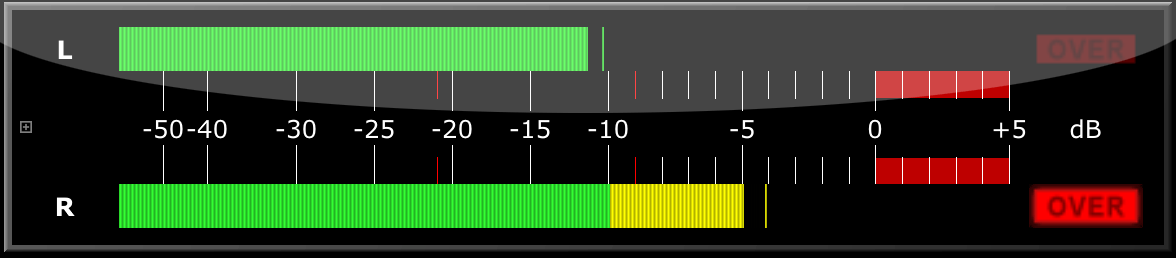
\includegraphics[width=\columnwidth]{ppmulator}%
                \end{figure}
            \end{columns}
            \pause
            \bigskip
            \bigskip
            \bigskip
            \textbf{related terms}: magnitude $\bullet$ intensity $\bullet$ envelope $\bullet$ level $\bullet$ volume $\bullet$ velocity $\bullet$ loudness
            
        \end{frame}

    \section[perception]{loudness perception}
        \begin{frame}{intensity, magnitude \& loudness}{human perception 1/2}
            perception has non-linear relation to magnitude/RMS:
            \begin{itemize}
                \item	model: logarithmic relation
                    \begin{equation*}
                        v_\mathrm{dB}(n) = 20\cdot\log_{10}\left(\frac{v(n)}{v_0}\right)
                    \end{equation*}
        

                    \begin{itemize}
                        \item	$v_0$: reference constant (\unit[0]{dB} point)
                            \begin{itemize}
                                \item   digital: $v_0 = 1$ $\Rightarrow \unit{dBFS}$
                                \item   sound pressure $v_0 = 20\cdot10^{-6}$ $\Rightarrow \unit{dBSPL}$
                            \end{itemize}
                        
                        \smallskip
                        \item	scaling	factor: \unit[1]{dB} $\approx$ JNDL for sound pressure level
                    \end{itemize}
            \end{itemize}
        \end{frame}
        
        \begin{frame}{intensity, magnitude \& loudness}{side note: level computation}
            \begin{itemize}
                \item if $v(n) = 0\quad\Rightarrow$: computation of $\log_{10}(0)$
                \item<2-> \textbf{work-arounds}
                    \begin{enumerate}[a]
                        \item	add constant $\epsilon$
                            \begin{equation*}
                                v_\mathrm{dB}(n) = 20\cdot\log_{10}(v(n) + \epsilon)
                            \end{equation*}
                            \only<2>{\vspace{-6mm}\figwithmatlab{LogEpsilon}}

                        \item<3->	add \textbf{if} statement	
                            \begin{equation*}
                                v_\mathrm{trunc}(n)  =   \left\{ 
                                            \begin{array}{ll} 
                                                v(n), & \text{if } v(n) \geq \epsilon \\
                                                \epsilon, & \text{otherwise }
                                            \end{array} 
                                            \right. 
                            \end{equation*}
                    \end{enumerate}
            \end{itemize}
        \end{frame}
        
        \begin{frame}{intensity, magnitude \& loudness}{human perception 2/2}
            \only<1-2>{
            \begin{itemize}
                \item   decibel scale is \textit{not} loudness scale:
                    \begin{itemize}
                        \item	equal-sized steps on the decibel scale not perceived as equal-sized loudness steps
                    \end{itemize}
                \bigskip
                \item<2>  perceptual phenomenon loudness depends on
                    \begin{itemize}
                        \item	frequency
                        \item	cochlear resolution
                        \item	masking effects
                    \end{itemize}
            \end{itemize}
            }
            \only<3>{
            \figwithmatlab{EqualLoudnessContours}
            }
        \end{frame}	
        

    \section[music]{loudness in music}
        \begin{frame}{intensity, magnitude \& loudness}{dynamics in music}
            \begin{itemize}
                \item	\textbf{score}:
                        \begin{itemize}
                            \item	only several rough dynamic steps,e.g.:\\ \emph{\textbf{pp}}, \textit{\textbf{p}}, \emph{\textbf{mf}}, \emph{\textbf{f}}, \emph{\textbf{ff}}
                            \item<1->	comparably vague instructions on volume modifications, e.g.:\\ \textsl{crescendo}, \textsl{decrescendo}, \emph{\textbf{sf}}
                            \item<1->	dynamics influenced by
                                    \begin{itemize}
                                        \item	instrumentation
                                        \item	timbre
                                        \item	number of voices
                                        \item	context and musical tension
                                    \end{itemize}
                        \end{itemize}
                \smallskip
                \item<2->	\textbf{MIDI}:
                        \begin{itemize}
                            \item	$128$ velocity steps
                            \item	no standardized relation to magnitude, power, \ldots
                        \end{itemize}
            \end{itemize}
        \end{frame}


    \section[features]{loudness features}
        \begin{frame}{intensity, magnitude \& loudness}{features: root mean square 1/2}
            \vspace{-6mm}
            \begin{equation*}
                v_{\mathrm{RMS}}(n) = \sqrt{\frac{1}{\mathcal{K}}\sum\limits_{i=i_{\mathrm{s}}(n)}^{i_{\mathrm{e}}(n)}{x(i)^2}}
            \end{equation*}
            \only<2>{
                \begin{itemize}
                    \item   value of this feature for the hypothetical prototype signals
                        \begin{itemize}
                            \item   silence
                            \item   sinusoidal (Amplitude $A$)
                            %\item   rect.\ white noise (Amplitude $A$)
                        \end{itemize}
                \end{itemize}
            }
            \only<3>{
                \vspace{-4mm}
                \figwithref{FeaturesTimeRms}{matlab source: \href{https://github.com/alexanderlerch/ACA-Slides/blob/master/matlab/displayFeatures.m}{matlab/displayFeatures.m}}
            }
            \vspace{50mm}
        \end{frame}
        \begin{frame}{intensity, magnitude \& loudness}{features: root mean square 2/2}
                \textbf{common variants}  (sample processing only):
                \begin{itemize}
                    \item<1->	reduce computational complexity
                        \begin{footnotesize}
                        \begin{eqnarray*}
                            v^2_{\mathrm{RMS}}(n) &=& \frac{x(i_{\mathrm{e}}(n))^2 - x(i_{\mathrm{s}}(n-1))^2}{i_{\mathrm{e}}(n)-i_{\mathrm{s}}(n) + 1} + v^2_{\mathrm{RMS}}(n-1) \\
                            v_{\mathrm{RMS}}(n)	&=& \sqrt{v^2_{\mathrm{RMS}}(n)}
                        \end{eqnarray*}
                        \end{footnotesize}
                    \smallskip
                    \item<2->	single pole approximation
                        \begin{footnotesize}
                        \begin{eqnarray*}
                            v_\mathrm{tmp}(i)	&=& \alpha\cdot v_\mathrm{tmp}(i-1) + (1-\alpha)\cdot x(i)^2\\
                            v^*_{\mathrm{RMS}}(i)		&=& \sqrt{v_\mathrm{tmp}(i)}
                        \end{eqnarray*}
                        \end{footnotesize}
                \end{itemize}
        \end{frame}
        \begin{frame}{intensity, magnitude \& loudness}{features: weighted root mean square}
            \begin{columns}
            \column{0.6\linewidth}
                \vspace{-8mm}
                \begin{figure}
                    \centering
                    \begin{footnotesize}
	\setcounter{iXOffset}{0}
	\setcounter{iYOffset}{5}
	\setcounter{iXBlockSize}{20}
	\setcounter{iYBlockSize}{16}
	\setcounter{iDistance}{5}
	\setcounter{iYBlockSizeDiv2}{8}
    \begin{picture}(57,26)


		\addtocounter{iYOffset}{\value{iYBlockSizeDiv2}}
		\addtocounter{iYOffset}{1}
        \put(\value{iXOffset},\value{iYOffset}){\footnotesize{\shortstack[c]{$x(i)$}}}
		\addtocounter{iYOffset}{-1}
		\addtocounter{iXOffset}{2}

        \put(\value{iXOffset},\value{iYOffset}){\vector(1,0){\value{iDistance}}}
		\addtocounter{iYOffset}{-\value{iYBlockSizeDiv2}}

		\addtocounter{iXOffset}{\value{iDistance}}
        \put(\value{iXOffset},\value{iYOffset}){\framebox(\value{iXBlockSize}, \value{iYBlockSize}){\footnotesize{\shortstack[c]{$H(z)$}}}}

		\addtocounter{iXOffset}{\value{iXBlockSize}}
		\addtocounter{iYOffset}{\value{iYBlockSizeDiv2}}
        \put(\value{iXOffset},\value{iYOffset}){\vector(1,0){\value{iDistance}}}
		\addtocounter{iYOffset}{-\value{iYBlockSizeDiv2}}

		\addtocounter{iXOffset}{\value{iDistance}}
        \put(\value{iXOffset},\value{iYOffset}){\framebox(\value{iXBlockSize}, \value{iYBlockSize}){\footnotesize{\shortstack[c]{$\mathrm{RMS}$}}}}

		\addtocounter{iXOffset}{\value{iXBlockSize}}
		\addtocounter{iYOffset}{\value{iYBlockSizeDiv2}}
        \put(\value{iXOffset},\value{iYOffset}){\vector(1,0){\value{iDistance}}}

        %text
		\addtocounter{iYOffset}{1}
		\addtocounter{iXOffset}{3}
        \put(\value{iXOffset},\value{iYOffset}){\footnotesize{\shortstack[c]{$v(n)$}}}

    \end{picture}
\end{footnotesize}

                \end{figure}
            \column{0.4\linewidth}
            $H(z)$:
            \begin{itemize}
                \item	A, B, C weighting
                \item	RLB (BS.1770)
                \item	\ldots
            \end{itemize}
            \end{columns}
            \vspace{-3mm}
            
            \only<2->{
            \figwithmatlab{LoudnessWeighting}
            }
        \end{frame}

         \begin{frame}{intensity, magnitude \& loudness}{features: peak envelope (max)}
            \vspace{-5mm}
            \begin{equation*}
                v_{\mathrm{Peak}}(n) = \max_{i_{\mathrm{s}}(n) \leq i \leq i_{\mathrm{e}}(n)}{|x(i)|} 
            \end{equation*}
            \only<2>{
                \vspace{-3mm}
                \figwithref{FeaturesTimePeakEnvelope}{matlab source: \href{https://github.com/alexanderlerch/ACA-Slides/blob/master/matlab/displayFeatures.m}{matlab/displayFeatures.m}}
            }
            \vspace{50mm}
        \end{frame}
        
        \begin{frame}{intensity, magnitude \& loudness}{features: peak envelope (PPM) 1/2}
            \begin{figure}
                \centering
                				\begin{footnotesize}
					\begin{picture}(100,40)(0,0)
			
						\put(-0.5,30){\circle{1}}
						\put(0,30){\vector(1,0){10}}
				
						\put(10,25){\framebox(10,10){}}
							\put(11,30){\line(1,0){8}}
							\put(15,26){\line(0,1){8}}
							\put(15,30){\line(1,1){4}}
							\put(15,30){\line(-1,1){4}}
									
						\put(20,30){\vector(1,0){5.4}}
			
						\put(25.2,28.5){\LARGE{$\oplus$}}
						
						\put(29.6,30){\vector(1,0){5.4}}
							
						\put(35,25){\framebox(10,10){}}
							\put(36,30){\line(1,0){8}}
							\put(40,26){\line(0,1){8}}
							\put(40,30){\line(1,1){4}}
						
						\put(45,30){\vector(1,0){5.4}}
			
						\put(50.2,28.5){\LARGE{$\otimes$}}
						
						\put(54.6,30){\vector(1,0){5.8}}
			
						\put(60.2,28.5){\LARGE{$\oplus$}}
						
						\put(64.6,30){\vector(1,0){5.8}}
			
						\put(70.2,28.5){\LARGE{$\oplus$}}
						
						\put(74.6,30){\vector(1,0){25.4}}
			
			
						\put(95,10){\vector(-1,0){5}}
							
						\put(80,5){\framebox(10,10){$z^{-1}$}}
			
						\put(80,10){\line(-1,0){52.5}}
			
			
			
						\put(95,30){\circle*{1}}
						\put(95,30){\line(0,-1){20}}
			
						\put(27.5,10){\vector(0,1){17.9}}
			
						\put(62.5,10){\circle*{1}}
						\put(62.5,10){\vector(0,1){17.9}}
			
						\put(72.5,10){\circle*{1}}
						\put(72.5,10){\vector(0,1){7.9}}
			
						\put(70.2,18.5){\LARGE{$\otimes$}}
			
						\put(72.5,22.1){\vector(0,1){5.8}}
						
						
						\put(0,34){\shortstack[c]{$x(i)$}}
						
						\put(21,34){\shortstack[c]{$|x(i)|$}}
						
						\put(29,26){\shortstack[c]{$-$}}
						
						\put(52,32.5){\shortstack[c]{$\alpha_\mathrm{AT}$}}
						
						\put(75,19){\shortstack[c]{$\lambda$}}
			
						\put(74,26){\shortstack[c]{$-$}}
						
						
						\put(95,34){\shortstack[c]{$v_{\mathrm{PPM}}(i)$}}
					\end{picture}
				\end{footnotesize}

            \end{figure}	
            \only<1>{\vspace{30mm}}
            \only<2->{
            \begin{itemize}
                \only<2-3>{
                \item \textbf{release state} ($|x(i)| < v_{\mathrm{PPM}}(i-1)\Rightarrow\lambda = \alpha_\mathrm{RT}$)
                    \invisible<2>{
                    \begin{eqnarray*}
                        v_{\mathrm{PPM}}(i) &=& v_{\mathrm{PPM}}(i-1) - \alpha_\mathrm{RT}\cdot v_{\mathrm{PPM}}(i-1)\nonumber\\
                                    &=& (1-\alpha_\mathrm{RT})\cdot v_{\mathrm{PPM}}(i-1) 
                    \end{eqnarray*}
                    }
                }
                \only<4-5>{
                \item \textbf{attack state} ($|x(i)| \geq v_{\mathrm{PPM}}(i-1)\Rightarrow\lambda = 0$)
                    \invisible<4>{
                    \begin{eqnarray*}
                        v_{\mathrm{PPM}}(i) &=& \alpha_\mathrm{AT}\cdot\big(|x(i)| - v_{\mathrm{PPM}}(i-1)\big) + v_{\mathrm{PPM}}(i-1)\nonumber\\
                                    &=& \alpha_\mathrm{AT}\cdot |x(i)| + (1-\alpha_\mathrm{AT})\cdot v_{\mathrm{PPM}}(i-1) 
                    \end{eqnarray*}
                    }
                }
            \end{itemize}
            }
        \end{frame}
        \begin{frame}{intensity, magnitude \& loudness}{features: peak envelope (PPM) 2/2}
            \vspace{-3mm}
            \figwithref{FeaturesTimePeakEnvelope}{matlab source: \href{https://github.com/alexanderlerch/ACA-Slides/blob/master/matlab/displayFeatures.m}{matlab/displayFeatures.m}}
            
            \vspace{-2mm}
            \begin{itemize}
                \item   gold: max per block
                \item   blue: PPM
            \end{itemize}
        \end{frame}
        
        \begin{frame}{intensity, magnitude \& loudness}{features: zwicker loudness}
            \vspace{-3mm}
    		\begin{figure}
            \scalebox{.8}
            {
                \centering
                \begin{footnotesize}

		\setcounter{iXOffset}{0}
		\setcounter{iYOffset}{5}
		\setcounter{iXBlockSize}{20}
		\setcounter{iYBlockSize}{16}
		\setcounter{iDistance}{5}
		
		\setcounter{iYBlockSizeDiv2}{13}
		
				\begin{picture}(120,21)

					\addtocounter{iYBlockSizeDiv2}{1}
					\put(\value{iXOffset}, \value{iYBlockSizeDiv2})
						{\footnotesize{\shortstack[c]{Stimulus}}}
					\addtocounter{iYBlockSizeDiv2}{-1}
					\addtocounter{iXOffset}{\value{iDistance}}
					\addtocounter{iXOffset}{\value{iDistance}}
					\put(\value{iXOffset}, \value{iYBlockSizeDiv2})
						{\vector(1,0){\value{iDistance}}}
					\addtocounter{iXOffset}{\value{iDistance}}
				
					\put(\value{iXOffset}, \value{iYOffset})
						{\framebox(\value{iXBlockSize}, \value{iYBlockSize}) {\shortstack[c]{Outer Ear\\Transfer\\ Function}}}
					\addtocounter{iXOffset}{\value{iXBlockSize}}
					\addtocounter{iYOffset}{\value{iDistance}}
					\put(\value{iXOffset}, \value{iYBlockSizeDiv2})
						{\vector(1,0){\value{iDistance}}}
					\addtocounter{iYOffset}{-\value{iDistance}}
					\addtocounter{iXOffset}{\value{iDistance}}
					
					\put(\value{iXOffset}, \value{iYOffset})
						{\framebox(\value{iXBlockSize}, \value{iYBlockSize}) {\shortstack[c]{Excitation\\ Patterns}}}
					\addtocounter{iXOffset}{\value{iXBlockSize}}
					\addtocounter{iYOffset}{\value{iDistance}}
					\put(\value{iXOffset}, \value{iYBlockSizeDiv2})
						{\vector(1,0){\value{iDistance}}}
					\addtocounter{iYOffset}{-\value{iDistance}}
					\addtocounter{iXOffset}{\value{iDistance}}
					
					\put(\value{iXOffset}, \value{iYOffset})
						{\framebox(\value{iXBlockSize}, \value{iYBlockSize}) {\shortstack[c]{Specific\\ Loudness}}}
					\addtocounter{iXOffset}{\value{iXBlockSize}}
					\addtocounter{iYOffset}{\value{iDistance}}
					\put(\value{iXOffset}, \value{iYBlockSizeDiv2})
						{\vector(1,0){\value{iDistance}}}
					\addtocounter{iYOffset}{-\value{iDistance}}
					\addtocounter{iXOffset}{\value{iDistance}}
					
					\put(\value{iXOffset}, \value{iYOffset})
						{\framebox(\value{iXBlockSize}, \value{iYBlockSize}) {\shortstack[c]{Overall\\ Loudness}}}
					\addtocounter{iXOffset}{\value{iXBlockSize}}
					\addtocounter{iYOffset}{\value{iDistance}}
					\put(\value{iXOffset}, \value{iYBlockSizeDiv2})
						{\vector(1,0){\value{iDistance}}}
					\addtocounter{iYOffset}{-\value{iDistance}}
					\addtocounter{iXOffset}{\value{iDistance}}
%					\put(\value{iXOffset}, \value{iYOffset})
%						{\footnotesize{\shortstack[c]{$v_\mathrm{Loud}$}}}
					\addtocounter{iYBlockSizeDiv2}{1}
					\put(\value{iXOffset}, \value{iYBlockSizeDiv2})
						{\footnotesize{\shortstack[c]{$v_\mathrm{Loud}$}}}
					\addtocounter{iYBlockSizeDiv2}{-1}
			
				\end{picture}
				\end{footnotesize}

            }
    		\end{figure}
            \vspace{-5mm}
            
            \uncover<2->{
            \begin{itemize}
                
                \item	
                \only<2>{ outer ear transfer function\footfullcite{hammershoi_methods_2002}
                \begin{figure}
                    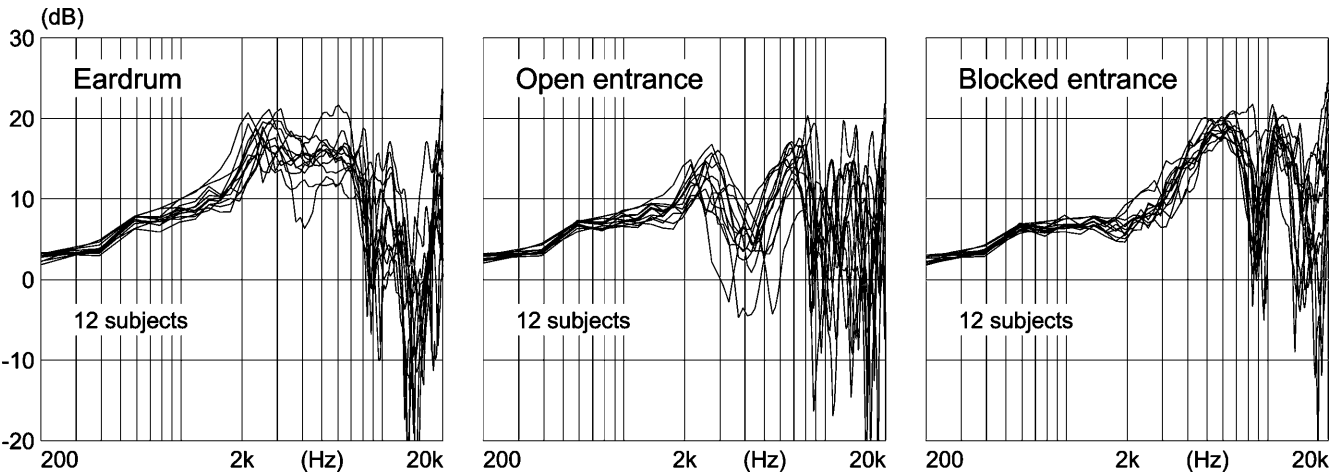
\includegraphics[scale=.25]{graph/OETF}
                \end{figure}
                }
                
                \only<3>{	excitation patterns\footfullcite{schleske_website}
                \begin{figure}
                    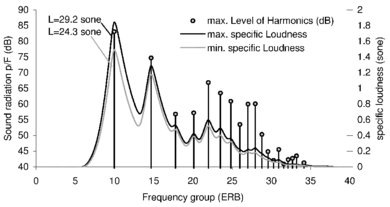
\includegraphics[scale=.5]{graph/excitationpatterns}
                \end{figure}
                }
                \only<4>{	specific loudness\footfullcite{specloudness_website}
                \begin{figure}
                    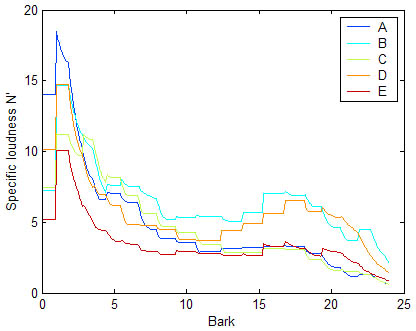
\includegraphics[scale=.35]{graph/specificloudness}
                \end{figure}
                }
                \only<5>{	overall loudness
                \[ v_\mathrm{loud} = \sum_{\forall i} z_i\]
                }
            \end{itemize}
            }
        \end{frame}

        \begin{frame}{intensity, magnitude \& loudness}{derived features}
            \begin{itemize}
                \item   number or ratio of pauses
                \item   dynamic range
                \item   other statistical features from (RMS) histogram
                \item   \ldots
            \end{itemize}
        \end{frame}
        
    \section{summary}
        \begin{frame}{summary}{lecture content}
            \begin{itemize}
                \item   \textbf{loudness perception}
                    \begin{itemize}
                        \item   nonlinear relation to magnitude or power
                        \item   depends also on frequency, level, and signal (masking)
                    \end{itemize}
                \bigskip
                \item   \textbf{typical features}
                    \begin{itemize}
                        \item   derived from envelope (peak, RMS, weighted RMS)
                        \item   derived from histogram (range, mode)
                    \end{itemize}
            \end{itemize}
            \inserticon{summary}
        \end{frame}
\end{document}
